% !TEX spellcheck = en_US



% ~~~~~~~~~~~~~~~~~~~~~~~~~~~~~~~~~~~~~~~ V
% (NC) 2026 Haluk Bingol
% github.com/halukbingol/LaTeX-Templates
%
% Licensees may copy, distribute, display, and perform the work and make derivative works 
% and remixes based on it only for non-commercial purposes. 
% ~~~~~~~~~~~~~~~~~~~~~~~~~~~~~~~~~~~~~~~ A




% =====================================================================
%  Internationalization in Java -- Senior Level: Architecture, Security and Delivery
%  ---------------------------------------------------------------------
%  Built on Template/hblibTemplate.tex with the libraries in ../../hblib/.
%  Programs, terminal sessions and their real outputs are in codeoutput/:
%     codeoutput/<Name>.java  a program        codeoutput/<Name>.sh   a session
%     codeoutput/<Name>/      the session's project folder
%     codeoutput/<Name>.txt   what it printed, made by:  bash run_examples.sh
% =====================================================================

\documentclass[aspectratio=169,10pt,compress]{beamer}

% ~~~~~~~~~~~~~~~~~~~~~~~~~~~~~~~~~~~~~~~~~~~~~~~~~~~~~~~~~~~~~~~~~ V hblib
	\usepackage{../../hblib/hblibPresentation} % lib presentation: theme, i/N, \hSection, algorithm2e, ...
	\usepackage{../../hblib/hblibCodeoutput} % lib code + output: \lstcode, \lstterminal, ...
	\usepackage{../../hblib/hblibDatastructures} % lib data structures: \hString, \hStack, \hQueue
% ~~~~~~~~~~~~~~~~~~~~~~~~~~~~~~~~~~~~~~~~~~~~~~~~~~~~~~~~~~~~~~~~~ A hblib


% xcolor, array (and the L{width} column), listings, tikz and algorithm2e come from the hblib libraries
\usepackage[T1]{fontenc}
\usepackage{lmodern}
\usepackage{booktabs}

\definecolor{gitred}{RGB}{240,80,50}
\newcommand{\win}{\textbf{Windows}}
\newcommand{\mac}{\textbf{macOS}}

% algorithm2e set-up (the package is loaded by hblibPresentation), as in the template
\SetAlCapFnt{\small}
\SetAlCapNameFnt{\small}
\DontPrintSemicolon

% .properties files (resource bundles)
\lstdefinelanguage{properties}{morecomment=[l]{\#}, morecomment=[l]{!}}

% ---------------------------------------------------------------------
\title{Internationalization in Java}
\subtitle{Senior Level: Architecture, Security and Delivery}
\author[Bingol]{Haluk O. Bingol}

\institute[FCIS]{
    Faculty of Computer and Information Sciences\\
    Yeditepe University
}
\date{
	{\tiny \hbTimeStamp}
}

\begin{document}




% ~~~~~~~~~~~~~~~~~~~~~~~~~~~~~~~~~~~~~~ V frm
\begin{frame}[t,fragile]
  \titlepage
\end{frame}
% ~~~~~~~~~~~~~~~~~~~~~~~~~~~~~~~~~~~~~~ A frm




% ~~~~~~~~~~~~~~~~~~~~~~~~~~~~~~~~~~~~~~ V frm
\begin{frame}[t,fragile] \frametitle{Outline}
  \begin{columns}[T]
    \begin{column}{0.48\textwidth}
      \tableofcontents[sections={1-3}, hideallsubsections]
    \end{column}
    \begin{column}{0.48\textwidth}
      \tableofcontents[sections={4-20}, hideallsubsections]
    \end{column}
  \end{columns}
\end{frame}
% ~~~~~~~~~~~~~~~~~~~~~~~~~~~~~~~~~~~~~~ A frm

% ~~~~~~~~~~~~~~~~~~~~~~~~~~~~~~~~~~~~~~ V
\hSection[Architecture]{Architecture}
% ~~~~~~~~~~~~~~~~~~~~~~~~~~~~~~~~~~~~~~ A




% ~~~~~~~~~~~~~~~~~~~~~~~~~~~~~~~~~~~~~~ V frm
\begin{frame}[t,fragile] \frametitle{Where internationalization lives in a system}
  \begin{center}
  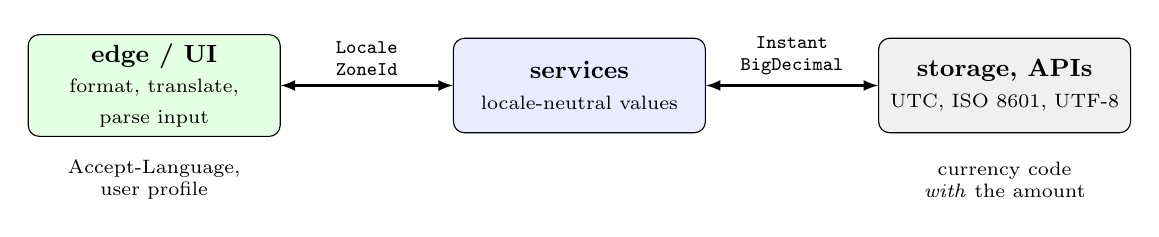
\begin{tikzpicture}[box/.style={draw, rounded corners, align=center, font=\small, minimum height=1.2cm, minimum width=3.2cm}]
    \node[box, fill=green!10] (ui) at (0,0) {\textbf{edge / UI}\\\scriptsize format, translate,\\\scriptsize parse input};
    \node[box, fill=blue!8] (svc) at (5.4,0) {\textbf{services}\\\scriptsize locale-neutral values};
    \node[box, fill=gray!12] (db) at (10.8,0) {\textbf{storage, APIs}\\\scriptsize UTC, ISO 8601, UTF-8};
    \draw[latex-latex, thick] (ui) -- node[above, font=\scriptsize, align=center] {\texttt{Locale}\\\texttt{ZoneId}} (svc);
    \draw[latex-latex, thick] (svc) -- node[above, font=\scriptsize, align=center] {\texttt{Instant}\\\texttt{BigDecimal}} (db);
    \node[font=\scriptsize, align=center] at (0,-1.2) {Accept-Language,\\user profile};
    \node[font=\scriptsize, align=center] at (10.8,-1.2) {currency code\\\emph{with} the amount};
  \end{tikzpicture}
  \end{center}
  \begin{itemize}\small
    \item Inside the system everything is \textbf{locale-neutral}: \texttt{Instant}, \texttt{BigDecimal} + ISO currency code, keys instead of texts.
    \item Only the \textbf{edge} formats and parses for a person; the locale and zone travel with the request, never as a global default.
    \item Logs, files, JSON, CSV, database: \texttt{Locale.ROOT}, UTF-8, ISO 8601, UTC.
  \end{itemize}
\end{frame}
% ~~~~~~~~~~~~~~~~~~~~~~~~~~~~~~~~~~~~~~ A frm

% ~~~~~~~~~~~~~~~~~~~~~~~~~~~~~~~~~~~~~~ V
\subsection[Negotiation]{Choosing the user's language}
% ~~~~~~~~~~~~~~~~~~~~~~~~~~~~~~~~~~~~~~ A




% ~~~~~~~~~~~~~~~~~~~~~~~~~~~~~~~~~~~~~~ V frm
\begin{frame}[t,fragile] \frametitle{Language negotiation}
% +++++++++++++++++++++++++++++++++++++++ V alg
%: -Alg. 
\begin{algorithm}[H]
  \caption{\textsc{Lookup}$(R, S)$ (RFC 4647, \texttt{Locale.lookup})}
  \KwIn{ranges $R = \langle r_{1}, \dots, r_{n} \rangle$ sorted by weight $q$; supported locales $S$}
  \KwOut{the best supported locale, or none}
  \ForEach{range $r$ in $R$ with $q > 0$}{
    $t \gets r$\;
    \While{$t$ is not empty}{
      \lIf{some $s \in S$ equals $t$}{\Return{$s$}}
      remove the last subtag of $t$		\tcp*{\texttt{de-CH} $\to$ \texttt{de}}
    }
  }
  \Return{none}\;
\end{algorithm}
% +++++++++++++++++++++++++++++++++++++++ A alg

\end{frame}
% ~~~~~~~~~~~~~~~~~~~~~~~~~~~~~~~~~~~~~~ A frm




% ~~~~~~~~~~~~~~~~~~~~~~~~~~~~~~~~~~~~~~ V frm
\begin{frame}[t,fragile] \frametitle{Accept-Language in Java}
  \lstcode[basicstyle=\ttfamily\tiny, firstline=5, firstnumber=5]{codeoutput/Negotiate.java}{Java}
  \uncover<2->{\lstterminal[basicstyle=\ttfamily\tiny]{codeoutput/Negotiate.txt}}

  \vspace{0.1em}
  \small
  \texttt{de-CH} falls back to \texttt{de}; French is not offered, so \texttt{en} wins; \texttt{ja-JP}: nothing, use the default.
\end{frame}
% ~~~~~~~~~~~~~~~~~~~~~~~~~~~~~~~~~~~~~~ A frm

% ~~~~~~~~~~~~~~~~~~~~~~~~~~~~~~~~~~~~~~ V
\hSection[Bundles]{Bundles at Scale}
% ~~~~~~~~~~~~~~~~~~~~~~~~~~~~~~~~~~~~~~ A

% ~~~~~~~~~~~~~~~~~~~~~~~~~~~~~~~~~~~~~~ V
\subsection[Modules]{Language packs as modules}
% ~~~~~~~~~~~~~~~~~~~~~~~~~~~~~~~~~~~~~~ A




% ~~~~~~~~~~~~~~~~~~~~~~~~~~~~~~~~~~~~~~ V frm
\begin{frame}[t,fragile] \frametitle{The application module}
  \lstcode[basicstyle=\ttfamily\tiny, numbers=none]{codeoutput/LanguagePack/src/app/module-info.java}{Java}
  \lstcode[basicstyle=\ttfamily\tiny, numbers=none]{codeoutput/LanguagePack/src/app/com/app/i18n/spi/MessagesProvider.java}{Java}
  \lstcode[basicstyle=\ttfamily\tiny, numbers=none, firstline=6]{codeoutput/LanguagePack/src/app/com/app/Main.java}{Java}
\end{frame}
% ~~~~~~~~~~~~~~~~~~~~~~~~~~~~~~~~~~~~~~ A frm




% ~~~~~~~~~~~~~~~~~~~~~~~~~~~~~~~~~~~~~~ V frm
\begin{frame}[t,fragile] \frametitle{The language pack module}
  \lstcode[basicstyle=\ttfamily\tiny, numbers=none]{codeoutput/LanguagePack/src/app.tr/module-info.java}{Java}
  \lstcode[basicstyle=\ttfamily\tiny, numbers=none]{codeoutput/LanguagePack/src/app.tr/com/app/tr/TurkishMessages.java}{Java}
  \small A pack is a module that \textbf{provides} the service the application \textbf{uses}.
\end{frame}
% ~~~~~~~~~~~~~~~~~~~~~~~~~~~~~~~~~~~~~~ A frm




% ~~~~~~~~~~~~~~~~~~~~~~~~~~~~~~~~~~~~~~ V frm
\begin{frame}[t,fragile] \frametitle{Adding a language without changing the application}
  \lstterminal[basicstyle=\ttfamily\tiny]{codeoutput/LanguagePack.txt}

  \vspace{0.1em}
  \small
  In a named module \texttt{getBundle} also asks the \texttt{ResourceBundleProvider} services. The Turkish pack is a separate
  module on the module path: present, Turkish; absent, English. Two modules may not share a package, so the pack uses its own.
\end{frame}
% ~~~~~~~~~~~~~~~~~~~~~~~~~~~~~~~~~~~~~~ A frm

% ~~~~~~~~~~~~~~~~~~~~~~~~~~~~~~~~~~~~~~ V
\subsection[Custom loading]{Custom loading}
% ~~~~~~~~~~~~~~~~~~~~~~~~~~~~~~~~~~~~~~ A




% ~~~~~~~~~~~~~~~~~~~~~~~~~~~~~~~~~~~~~~ V frm
\begin{frame}[t,fragile] \frametitle{Bundles from a folder, reloaded}
  \begin{columns}[T]
    \begin{column}{0.64\textwidth}
      \lstcode[basicstyle=\ttfamily\tiny, firstline=12, firstnumber=12]{codeoutput/Reload/Reload.java}{Java}
    \end{column}
    \begin{column}{0.34\textwidth}
      \uncover<2->{\lstterminal[basicstyle=\ttfamily\tiny]{codeoutput/Reload.txt}}
      \uncover<2->{\small A \texttt{Control} decides \emph{where} bundles come from (files, database, a translation server)
      and \emph{how long} they are cached. Translators can fix texts without a new release.}
    \end{column}
  \end{columns}
\end{frame}
% ~~~~~~~~~~~~~~~~~~~~~~~~~~~~~~~~~~~~~~ A frm

% ~~~~~~~~~~~~~~~~~~~~~~~~~~~~~~~~~~~~~~ V
\subsection[Checks]{Checking translations}
% ~~~~~~~~~~~~~~~~~~~~~~~~~~~~~~~~~~~~~~ A




% ~~~~~~~~~~~~~~~~~~~~~~~~~~~~~~~~~~~~~~ V frm
\begin{frame}[t,fragile] \frametitle{Three bundles, three mistakes}
  \lstcode[basicstyle=\ttfamily\tiny, numbers=none]{codeoutput/BundleCheck/Messages.properties}{properties}
  \lstcode[basicstyle=\ttfamily\tiny, numbers=none]{codeoutput/BundleCheck/Messages_tr.properties}{properties}
  \lstcode[basicstyle=\ttfamily\tiny, numbers=none]{codeoutput/BundleCheck/Messages_de.properties}{properties}
  \small Can you find them? \uncover<2->{German has an unknown key, Turkish misses \texttt{bye}, and Turkish \texttt{items}
  lost \texttt{\{1\}}: the city would silently disappear.}
\end{frame}
% ~~~~~~~~~~~~~~~~~~~~~~~~~~~~~~~~~~~~~~ A frm




% ~~~~~~~~~~~~~~~~~~~~~~~~~~~~~~~~~~~~~~ V frm
\begin{frame}[t,fragile] \frametitle{Checking translations automatically (run it in CI)}
  \lstcode[basicstyle=\ttfamily\tiny, firstline=20, firstnumber=20]{codeoutput/BundleCheck/BundleCheck.java}{Java}
  \uncover<2->{\lstterminal[basicstyle=\ttfamily\tiny]{codeoutput/BundleCheck.txt}}
\end{frame}
% ~~~~~~~~~~~~~~~~~~~~~~~~~~~~~~~~~~~~~~ A frm

% ~~~~~~~~~~~~~~~~~~~~~~~~~~~~~~~~~~~~~~ V
\subsection[Runtime]{Locale data in the runtime}
% ~~~~~~~~~~~~~~~~~~~~~~~~~~~~~~~~~~~~~~ A




% ~~~~~~~~~~~~~~~~~~~~~~~~~~~~~~~~~~~~~~ V frm
\begin{frame}[t,fragile] \frametitle{Smaller runtimes: \texttt{jlink --include-locales}}
  \lstterminal[basicstyle=\ttfamily\tiny]{codeoutput/Jlink.txt}

  \vspace{0.1em}
  \small
  Only \texttt{java.base} has English data; all other locales are in \texttt{jdk.localedata}. Without it Turkish silently
  falls back to the \emph{root} format. \texttt{--include-locales=en,tr} keeps exactly what you ship (German is gone).
\end{frame}
% ~~~~~~~~~~~~~~~~~~~~~~~~~~~~~~~~~~~~~~ A frm

% ~~~~~~~~~~~~~~~~~~~~~~~~~~~~~~~~~~~~~~ V
\hSection[Security]{Security}
% ~~~~~~~~~~~~~~~~~~~~~~~~~~~~~~~~~~~~~~ A

% ~~~~~~~~~~~~~~~~~~~~~~~~~~~~~~~~~~~~~~ V
\subsection[Case]{Case and identity}
% ~~~~~~~~~~~~~~~~~~~~~~~~~~~~~~~~~~~~~~ A




% ~~~~~~~~~~~~~~~~~~~~~~~~~~~~~~~~~~~~~~ V frm
\begin{frame}[t,fragile] \frametitle{A real attack: the Turkish i}
  \begin{columns}[T]
    \begin{column}{0.6\textwidth}
      \lstcode[basicstyle=\ttfamily\tiny]{codeoutput/Register/Register.java}{Java}
    \end{column}
    \begin{column}{0.38\textwidth}
      \uncover<2->{\lstterminal[basicstyle=\ttfamily\scriptsize]{codeoutput/Register.txt}}
    \end{column}
  \end{columns}

  \vspace{0.1em}
  \small On a server whose default locale is Turkish, \texttt{"admin".toUpperCase()} is \texttt{"ADMİN"}: the check passes and an
  attacker owns the name \texttt{admin}. Security checks must use \texttt{Locale.ROOT} (or compare canonical keys).
\end{frame}
% ~~~~~~~~~~~~~~~~~~~~~~~~~~~~~~~~~~~~~~ A frm




% ~~~~~~~~~~~~~~~~~~~~~~~~~~~~~~~~~~~~~~ V frm
\begin{frame}[t,fragile] \frametitle{Look-alike user names}
  \begin{columns}[T]
    \begin{column}{0.54\textwidth}
      \lstcode[basicstyle=\ttfamily\tiny, firstline=4, firstnumber=4]{codeoutput/Usernames.java}{Java}
    \end{column}
    \begin{column}{0.44\textwidth}
      \uncover<2->{\lstterminal[basicstyle=\ttfamily\tiny]{codeoutput/Usernames.txt}}
    \end{column}
  \end{columns}

  \vspace{0.1em}
  \small
  NFKC + \texttt{ROOT} lower case catches the full-width \emph{a} (FF41) and the Roman numeral \emph{m} (217F).
  The Cyrillic \emph{a} (430) stays different: \emph{confusables} need a separate check (Unicode TR 39, ICU \texttt{SpoofChecker}).
\end{frame}
% ~~~~~~~~~~~~~~~~~~~~~~~~~~~~~~~~~~~~~~ A frm




% ~~~~~~~~~~~~~~~~~~~~~~~~~~~~~~~~~~~~~~ V frm
\begin{frame}[t,fragile] \frametitle{More traps}
  \begin{columns}[T]
    \begin{column}{0.48\textwidth}
      \begin{block}{Invisible and direction characters}
        \small Characters such as U+202E (right-to-left override) and U+200B (zero-width space) change how text
        \emph{looks} without changing what it \emph{is}: fake file names (\texttt{gpj.exe} shown as \texttt{exe.jpg}),
        hidden code in reviews (\emph{Trojan Source}, CVE-2021-42574). Strip or reject them in identifiers.
      \end{block}
    \end{column}
    \begin{column}{0.48\textwidth}
      \begin{block}{Normalize, then validate}
        \small Validate \textbf{after} normalizing and decoding, never before: otherwise \texttt{..}, \texttt{/},
        \texttt{<} can come back in another form. Keep one canonical form (NFC, UTF-8) in storage.
      \end{block}
      \begin{block}{Untrusted patterns}
        \small A translation is code: \texttt{MessageFormat} patterns from outside can break formatting.
        Validate bundles (previous section) before deploying them.
      \end{block}
    \end{column}
  \end{columns}
\end{frame}
% ~~~~~~~~~~~~~~~~~~~~~~~~~~~~~~~~~~~~~~ A frm

% ~~~~~~~~~~~~~~~~~~~~~~~~~~~~~~~~~~~~~~ V
\subsection[Machine formats]{Machine-readable formats}
% ~~~~~~~~~~~~~~~~~~~~~~~~~~~~~~~~~~~~~~ A




% ~~~~~~~~~~~~~~~~~~~~~~~~~~~~~~~~~~~~~~ V frm
\begin{frame}[t,fragile] \frametitle{Default locale in a data file}
  \begin{columns}[T]
    \begin{column}{0.52\textwidth}
      \lstcode[basicstyle=\ttfamily\tiny]{codeoutput/Csv/Report.java}{Java}
    \end{column}
    \begin{column}{0.46\textwidth}
      \uncover<2->{\lstterminal[basicstyle=\ttfamily\scriptsize]{codeoutput/Csv.txt}}
    \end{column}
  \end{columns}

  \vspace{0.1em}
  \small The Turkish server writes \texttt{12,50}: the CSV row now has 4 fields, and the next program reads the price as 12.
  Every machine format needs \texttt{Locale.ROOT}: \texttt{String.format(Locale.ROOT, ...)}, \texttt{toUpperCase(Locale.ROOT)}.
\end{frame}
% ~~~~~~~~~~~~~~~~~~~~~~~~~~~~~~~~~~~~~~ A frm




% ~~~~~~~~~~~~~~~~~~~~~~~~~~~~~~~~~~~~~~ V frm
\begin{frame}[t,fragile] \frametitle{Encodings come from the environment}
  \lstterminal[basicstyle=\ttfamily\tiny]{codeoutput/Encodings.txt}

  \vspace{0.1em}
  \small
  \texttt{file.encoding} (default charset) is UTF-8 since Java 18. \texttt{native.encoding}, \texttt{sun.jnu.encoding}
  (file names) and \texttt{stdout.encoding} still follow the operating system: a Latin-5 server writes Latin-5 to the
  console. Name the charset in every \texttt{Reader}, \texttt{Writer}, \texttt{getBytes}.
\end{frame}
% ~~~~~~~~~~~~~~~~~~~~~~~~~~~~~~~~~~~~~~ A frm

% ~~~~~~~~~~~~~~~~~~~~~~~~~~~~~~~~~~~~~~ V
\hSection[Delivery]{Delivery and Operations}
% ~~~~~~~~~~~~~~~~~~~~~~~~~~~~~~~~~~~~~~ A




% ~~~~~~~~~~~~~~~~~~~~~~~~~~~~~~~~~~~~~~ V frm
\begin{frame}[t,fragile] \frametitle{Servers and containers}
  \begin{columns}[T]
    \begin{column}{0.5\textwidth}


% +++++++++++++++++++++++++++++++++++++++ V lst
%: -Lst.
\begin{lstlisting}[style=codesnippet, language=bash, basicstyle=\ttfamily\scriptsize]
FROM eclipse-temurin:21-jre
ENV LANG=C.UTF-8 TZ=UTC
COPY app.jar /app/app.jar
ENTRYPOINT ["java", "-Duser.language=en", \
  "-Duser.country=US", "-Duser.timezone=UTC", \
  "-jar", "/app/app.jar"]
\end{lstlisting}
% +++++++++++++++++++++++++++++++++++++++ A lst


      \small \hRemark{Not run here.} Same on \win{} and \mac{} with Docker Desktop.
    \end{column}
    \begin{column}{0.46\textwidth}
      \begin{itemize}\small
        \item Make the server's defaults \textbf{explicit}: a container without \texttt{LANG} differs from a laptop.
        \item The defaults should never matter: pass the user's locale and zone through the code.
        \item Keep the JDK updated: CLDR data and the time zone database come with it
          (\texttt{tzupdater} can patch only the zones).
        \item Log in English with \texttt{Locale.ROOT}; show the user a translated message with an error code.
      \end{itemize}
    \end{column}
  \end{columns}
\end{frame}
% ~~~~~~~~~~~~~~~~~~~~~~~~~~~~~~~~~~~~~~ A frm




% ~~~~~~~~~~~~~~~~~~~~~~~~~~~~~~~~~~~~~~ V frm
\begin{frame}[t,fragile] \frametitle{The translation workflow}
  \begin{center}
  \begin{tikzpicture}[st/.style={draw, rounded corners, align=center, font=\small, minimum width=2.6cm, minimum height=1.1cm}, node distance=0.6cm]
    \node[st, fill=blue!8] (dev) {developer\\\scriptsize adds key + English};
    \node[st, fill=gray!12, right=of dev] (ci) {CI\\\scriptsize checks, pseudo-loc};
    \node[st, fill=orange!12, right=of ci] (tms) {translation system\\\scriptsize XLIFF, memory};
    \node[st, fill=green!12, right=of tms] (rel) {release\\\scriptsize or language pack};
    \draw[-latex, thick] (dev) -- (ci); \draw[-latex, thick] (ci) -- (tms); \draw[-latex, thick] (tms) -- (rel);
  \end{tikzpicture}
  \end{center}
  \begin{itemize}\small
    \item Give translators \textbf{context}: a comment per key, a screenshot, the meaning of each \texttt{\{n\}}.
    \item Keys name the meaning (\texttt{order.items.count}), not the English words.
    \item One key per sentence; never reuse a key in two places (``Open'' a file vs.\ ``Open'' as a state).
    \item Tools: XLIFF files, translation memories, platforms like Weblate or Crowdin; review in the running product.
  \end{itemize}
\end{frame}
% ~~~~~~~~~~~~~~~~~~~~~~~~~~~~~~~~~~~~~~ A frm

% ~~~~~~~~~~~~~~~~~~~~~~~~~~~~~~~~~~~~~~ V
\hSection[Summary]{Summary}
% ~~~~~~~~~~~~~~~~~~~~~~~~~~~~~~~~~~~~~~ A




% ~~~~~~~~~~~~~~~~~~~~~~~~~~~~~~~~~~~~~~ V frm
\begin{frame}[t,fragile] \frametitle{Checklist for a product}
  \begin{columns}[T]
    \begin{column}{0.48\textwidth}
      \begin{block}{Design}
        \small
        \begin{itemize}
          \item locale-neutral core, formatting at the edge
          \item locale and zone per request / user, not global
          \item all machine formats with \texttt{Locale.ROOT}, UTF-8, ISO 8601
          \item language packs or reloadable bundles
        \end{itemize}
      \end{block}
    \end{column}
    \begin{column}{0.48\textwidth}
      \begin{block}{Quality and security}
        \small
        \begin{itemize}
          \item bundle checks and pseudo-localization in CI
          \item tests in \texttt{tr}, \texttt{de}, a right-to-left locale, several zones
          \item canonical keys (NFKC + ROOT) for identities
          \item explicit server defaults; JDK updates for CLDR and tzdata
        \end{itemize}
      \end{block}
    \end{column}
  \end{columns}
\end{frame}
% ~~~~~~~~~~~~~~~~~~~~~~~~~~~~~~~~~~~~~~ A frm




% ~~~~~~~~~~~~~~~~~~~~~~~~~~~~~~~~~~~~~~ V frm
\begin{frame}[t,fragile] \frametitle{Projects}
  \begin{enumerate}\small
    \item Build a small web service (\texttt{com.sun.net.httpserver}) that answers in the language of
      \texttt{Accept-Language} and formats money and dates for it.
    \item Turn the sophomore shop into modules with a German language pack provided as a separate module.
    \item Extend \texttt{BundleCheck}: report apostrophe problems and \texttt{choice} patterns that do not parse; run it in CI.
    \item Write a \texttt{ResourceBundle.Control} that reads translations from a database table and reloads every minute.
    \item Audit an open-source Java project for \texttt{toUpperCase()}/\texttt{toLowerCase()}/\texttt{String.format} without a locale.
    \item Measure the size and start-up time of \texttt{jlink} images with all locales vs.\ only yours.
  \end{enumerate}
\end{frame}
% ~~~~~~~~~~~~~~~~~~~~~~~~~~~~~~~~~~~~~~ A frm




% ~~~~~~~~~~~~~~~~~~~~~~~~~~~~~~~~~~~~~~ V frm
\begin{frame}[t,fragile]
	\begin{center}
		\vspace{4cm}
		\hRemark{\Huge Questions?}
	\end{center}
\end{frame}
% ~~~~~~~~~~~~~~~~~~~~~~~~~~~~~~~~~~~~~~ A frm



\end{document}
